\subsection{Чтение за пределами массива}

Итак, индексация массива --- это просто \IT{массив\lbrack{}индекс\rbrack}.  % TODO1 как-то плохо отображаются []
Если вы присмотритесь к коду, в цикле печати значений массива через \printf вы 
не увидите проверок индекса, \IT{меньше ли он двадцати?} 
А что будет если он будет 20 или больше? 
Эта одна из особенностей \CCpp, за которую их, собственно, и ругают.

Вот код, который и компилируется и работает:

\lstinputlisting{patterns/13_arrays/2_BO/r.c}

Вот результат компиляции в (MSVC 2008):

\lstinputlisting[caption=\NonOptimizing MSVC 2008]{patterns/13_arrays/2_BO/r_msvc.asm}

Данный код при запуске выдал вот такой результат:

\begin{figure}[h]
\centering
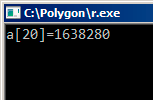
\includegraphics[scale=\NormalScale]{patterns/13_arrays/2_BO/olly_r3.png}
\caption{\olly: вывод в консоль}
\label{fig:array_BO_olly_r3}
\end{figure}

Это просто \IT{что-то}, что волею случая лежало в стеке рядом с массивом, 
через 80 байт от его первого элемента.

\clearpage
\myindex{\olly}
Попробуем узнать в \olly, что это за значение.
Загружаем и находим это значение, находящееся точно после последнего элемента массива:

\begin{figure}[H]
\centering
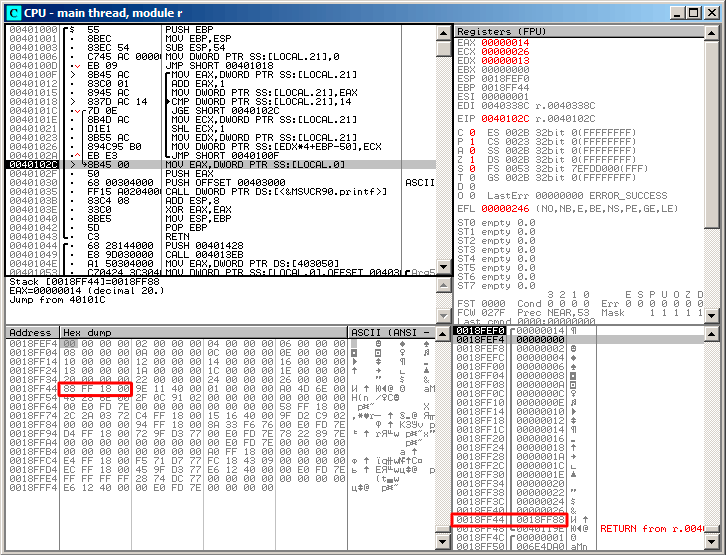
\includegraphics[scale=\FigScale]{patterns/13_arrays/2_BO/olly_r1.png}
\caption{\olly: чтение 20-го элемента и вызов \printf}
\label{fig:array_BO_olly_r1}
\end{figure}

Что это за значение? 
Судя по разметке стека, это сохраненное значение регистра EBP.
\clearpage
Трассируем далее, и видим, как оно восстанавливается:

\begin{figure}[H]
\centering
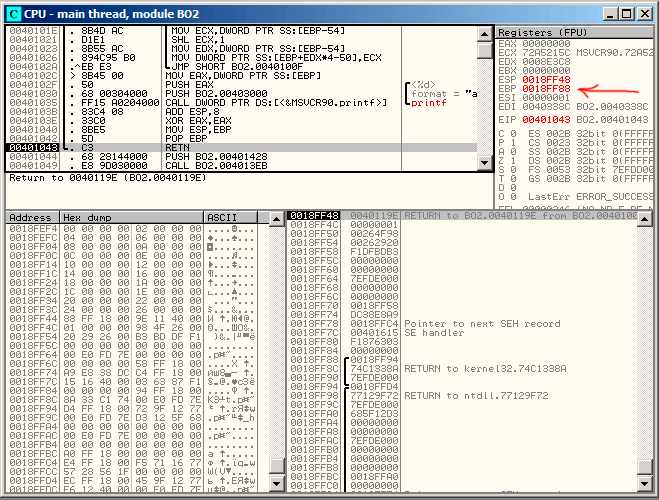
\includegraphics[scale=\FigScale]{patterns/13_arrays/2_BO/olly_r2.png}
\caption{\olly: восстановление EBP}
\label{fig:array_BO_olly_r2}
\end{figure}

Действительно, а как могло бы быть иначе? Компилятор мог бы встроить какой-то код, 
каждый раз проверяющий индекс на соответствие пределам массива, как в языках программирования 
более высокого уровня\footnote{Java, Python, итд.}, что делало бы запускаемый код медленнее.

